% ---
% title: 中文排版示例：《论语》与《大学》
% author: Mejistus
% ---
\usetikzlibrary{arrows.meta,positioning}

\begin{abstract}
这份文档借两部经典的开篇，演示 hatex 的中文排版：引文与脚注、原文与译文的双栏对照、列表与表格、TikZ 图、数学公式与命题，以及参考文献。
正文含有中文时，“图”“表”“命题”“证明”“参考文献”等名称会自动换成中文；源文件里中文之间的换行，也不会在网页上留下多余的空格。
\end{abstract}

\section{引文与脚注：《论语·学而》}\label{sec:lunyu}
《论语》是孔子弟子及再传弟子记录孔子言行的语录体著作，共二十篇~\cite{yang1980}。
首篇《学而》的第一章只有三句：
\begin{quote}
子曰：“学而时习之，不亦说\footnote{说（yuè）：同“悦”，喜悦。}乎？有朋自远方来，不亦乐乎？人不知而不愠\footnote{愠（yùn）：恼怒，怨恨。}，不亦君子乎？”
\end{quote}
引文用 \texttt{quote} 环境，注释用 \verb|\footnote|：编号自动生成并汇总到文末，点击编号可以来回跳转。

\subsection{原文与译文对照}\label{sec:parallel}
下面用 \texttt{multicols} 把原文与译文并排，\verb|\columnbreak| 指定换栏的位置；屏幕较窄时自动合为一栏。
\begin{multicols}{2}
\textbf{原文}

学而时习之，不亦说乎？

有朋自远方来，不亦乐乎？

人不知而不愠，不亦君子乎？
\columnbreak

\textbf{译文}

学了之后时常温习、练习，不也很愉快吗？

有志同道合的人从远方来，不也很快乐吗？

别人不了解我，我却不恼怒，不也是君子吗？
\end{multicols}

\section{《大学》：三纲领与八条目}\label{sec:daxue}
《大学》原是《礼记》的第四十二篇。南宋朱熹把它和《中庸》从《礼记》中抽出，与《论语》《孟子》合为“四书”，作《四书章句集注》~\cite{zhu1983}，四书之名由此确立（\autoref{tab:sishu}）。
其开篇为：
\begin{quote}
大学之道，在明明德，在亲民，在止于至善。知止而后有定，定而后能静，静而后能安，安而后能虑，虑而后能得。物有本末，事有终始，知所先后，则近道矣。
\end{quote}
第一句提出的三项宗旨，后世称为“三纲领”：
\begin{description}
  \item[明明德] 彰明人本有的光明德性；
  \item[亲民] 朱熹读作“新民”，使人弃旧图新；
  \item[止于至善] 达到并守住最完善的境地。
\end{description}
接下来一段讲实现它们的次第：
\begin{quote}
古之欲明明德于天下者，先治其国；欲治其国者，先齐其家；欲齐其家者，先修其身；欲修其身者，先正其心；欲正其心者，先诚其意；欲诚其意者，先致其知，致知在格物。
\end{quote}
由此归纳出的格物、致知、诚意、正心、修身、齐家、治国、平天下，称为“八条目”。
它们环环相扣，而“自天子以至于庶人，壹是皆以修身为本”，见\autoref{fig:tiaomu}。

\begin{figure}[htbp]
  \centering
  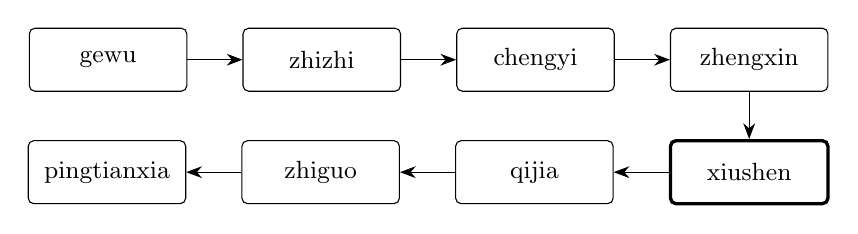
\begin{tikzpicture}[node distance=6mm and 7mm, >={Stealth[length=2mm]},
      stage/.style={draw, rounded corners=2pt, minimum width=20mm, minimum height=8mm, font=\small}]
    \node[stage] (gewu) {gewu};
    \node[stage, right=of gewu] (zhizhi) {zhizhi};
    \node[stage, right=of zhizhi] (chengyi) {chengyi};
    \node[stage, right=of chengyi] (zhengxin) {zhengxin};
    \node[stage, below=of zhengxin, very thick] (xiushen) {xiushen};
    \node[stage, left=of xiushen] (qijia) {qijia};
    \node[stage, left=of qijia] (zhiguo) {zhiguo};
    \node[stage, left=of zhiguo] (ping) {pingtianxia};
    \draw[->] (gewu) -- (zhizhi);
    \draw[->] (zhizhi) -- (chengyi);
    \draw[->] (chengyi) -- (zhengxin);
    \draw[->] (zhengxin) -- (xiushen);
    \draw[->] (xiushen) -- (qijia);
    \draw[->] (qijia) -- (zhiguo);
    \draw[->] (zhiguo) -- (ping);
  \end{tikzpicture}
  \caption{八条目的次第，“修身”一格加粗。图内文字用拼音：TikZ 由 plain \TeX{} 编译，没有中文字体，图中只能写 ASCII 字符。}\label{fig:tiaomu}
\end{figure}

\begin{table}[htbp]
  \centering
  \caption{四书概览。标“相传”的作者归属，历来有不同说法。}\label{tab:sishu}
  \begin{tabular}{llll}
    \toprule
    书名 & 篇数 & 作者或编者 & 来源 \\
    \midrule
    《大学》 & 1 & 相传为曾子 & 《礼记》第四十二篇 \\
    《中庸》 & 1 & 相传为子思 & 《礼记》第三十一篇 \\
    《论语》 & 20 & 孔子弟子及再传弟子 & 单独成书 \\
    《孟子》 & 7 & 孟子及其弟子 & 单独成书 \\
    \bottomrule
  \end{tabular}
\end{table}

\section{数学与中文混排：雉兔同笼}\label{sec:math}
《孙子算经》卷下有一道流传很广的题目~\cite{qian1963}：
\begin{quote}
今有雉兔同笼，上有三十五头，下有九十四足。问雉兔各几何？
\end{quote}
设雉有 $x$ 只、兔有 $y$ 只，由头数与足数得
\begin{equation}\label{eq:cage}
  \begin{cases} x + y = 35, \\ 2x + 4y = 94. \end{cases}
\end{equation}

\begin{proposition}[雉兔同笼]\label{prop:cage}
方程组~\eqref{eq:cage} 有唯一解 $x = 23$，$y = 12$，即雉二十三只、兔十二只。
\end{proposition}

\begin{proof}
第二式减去第一式的两倍，得 $2y = 24$，所以 $y = 12$，代入第一式得 $x = 23$。
系数行列式 $\begin{vmatrix} 1 & 1 \\ 2 & 4 \end{vmatrix} = 2 \neq 0$，故解唯一。
\end{proof}

原书的“术”更简洁：“上置头，下置足，半其足，以头除足，以足除头，即得。”这里的“除”是减的意思。
足数减半得 $94 / 2 = 47$，此时每只雉计 $1$、每只兔计 $2$，比头数多出的 $47 - 35 = 12$ 正是兔数，余下的 $35 - 12 = 23$ 是雉数，与命题~\ref{prop:cage} 一致。

\section{排版要点}\label{sec:notes}
\begin{itemize}
  \item 标点直接使用全角字符：“引号”、书名号《》、破折号——、省略号……都按原样显示。
  \item 中文之间的换行不产生空格，源文件可以一句一行，便于修改和比对。
  \item 图、表、命题、证明、参考文献等名称随正文自动中文化，\verb|\autoref| 生成“图~1”“表~1”。
  \item 字体由页面指定。本页用系统自带的宋体（Songti SC、Noto Serif CJK 等），hatex 本身不附带字体。
\end{itemize}

\begin{thebibliography}{9}
  \bibitem{yang1980} 杨伯峻. 论语译注[M]. 北京: 中华书局, 1980.
  \bibitem{zhu1983} 朱熹. 四书章句集注[M]. 北京: 中华书局, 1983.
  \bibitem{qian1963} 钱宝琮, 校点. 算经十书[M]. 北京: 中华书局, 1963.
\end{thebibliography}
